\chapter{Les émotions dans la parole}
\label{chapitre1}
"Chacun sait ce qu’est une émotion, jusqu’à ce qu’on lui demande d’en donner une définition. A ce moment-là, il semble que plus personne ne sache." (Fehr \& Russell, 1984)

 \section{Définition de l'émotion}
L'étude de l'émotion humaine est à la croisée de plusieurs domaines dont notamment la psychologie, la physiologie et la linguistique. Sa définition et sa caractérisation est encore aujourd'hui source d'études. En effet, il n'y a pas de consensus clair et établie sur une définition et une théorie qui prime sur les autres~\cite{Kleinginna1981,Strongman1996}. Néanmoins les scientifiques s'accordent à dire que les émotions sont des facteurs explicatifs des comportements de l'homme.

La définition de l'émotion est exprimée différemment en fonction des domaines d'étude. Pour le grand public, le dictionnaire Le Robert (www.shorturl.at/dsyNV) définit trois sens du mot émotion :
\begin{itemize}
    \item État affectif intense, caractérisé par des troubles divers (pâleur, accélération du pouls, etc.). Par exemple : Être paralysé par l'émotion ; Tu nous as donné des émotions, tu nous as fait peur (familier).
    \item État affectif, plaisir ou douleur, nettement prononcé.
    \item Sensibilité. Par exemple : Interpréter une œuvre avec émotion.
\end{itemize}
Au sein de cette thèse, nous considérons l'émotion selon la deuxième définition : l'émotion est un état temporaire dans lequel se trouve une personne, causée par un sentiment vif ressenti habituellement en réponse à une stimulation de l'environnement. Ce concept assez général regroupe une multitude d'états qui peuvent aller de la joie à la tristesse en passant par la peur et la colère par exemple. De nombreuses théories ont été présentées au fil des siècles pour définir l'émotion.

\subsection{Frise historique des théories de l'émotion}
\begin{figure}
  \centering
  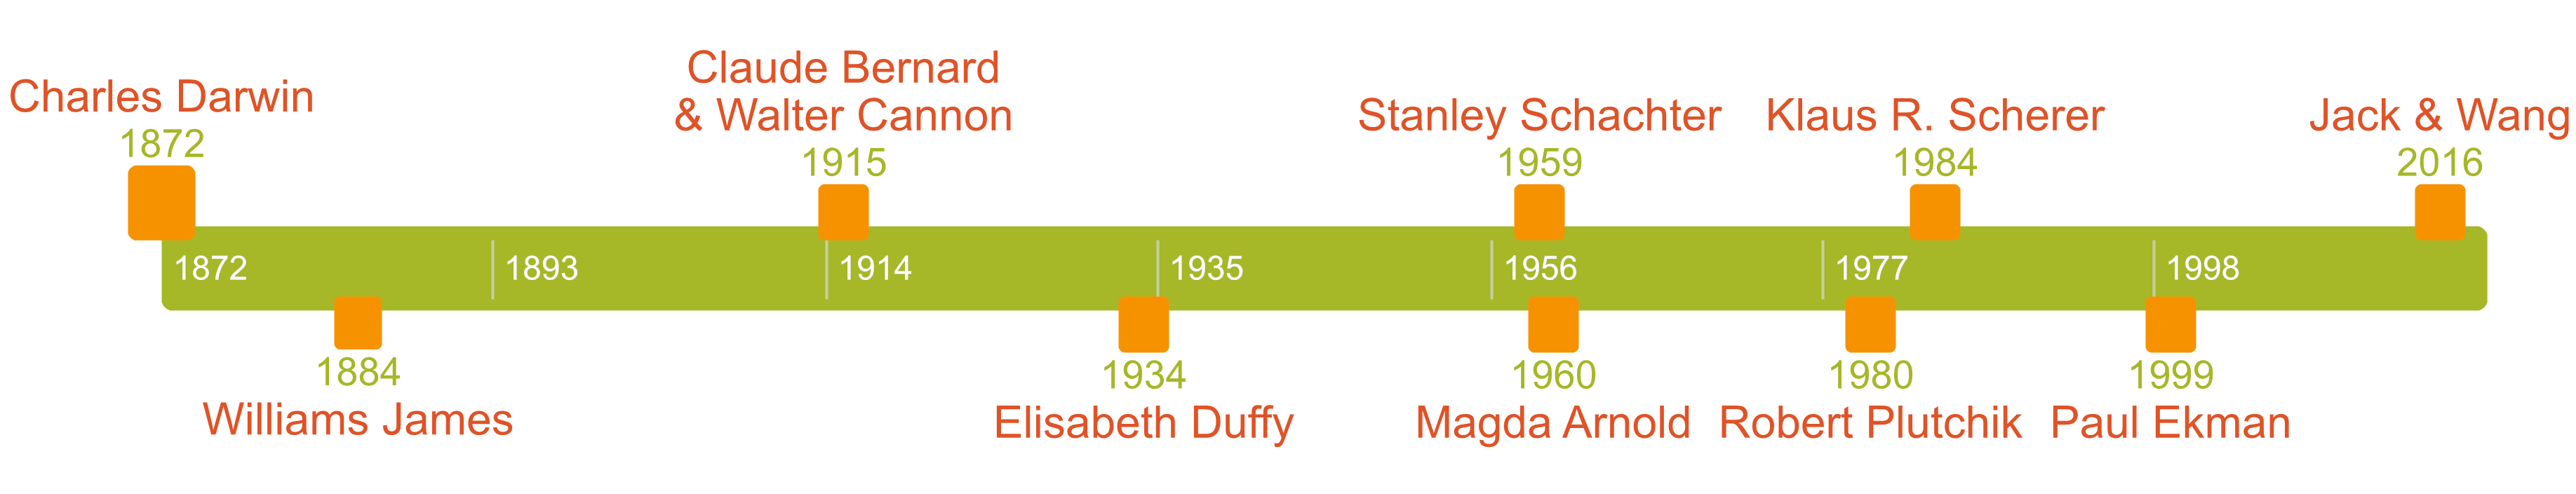
\includegraphics[width=16cm]{./Chapitre1/figures/friseHisto.png}
  \caption{Frise chronologique des grandes théories des émotions selon leur première date de parution}
  \label{fig:Circumplex}
\end{figure}


L'émotion et les états émotionnels, non content de ne pas avoir une unique définition, ont évolués dans leur caractérisation au fil du temps. Les premières mentions scientifiques de l'émotion nous viennent d'Aristote qui, au 4e siècle, définit l'Être comme une combinaison d'émotion et de raison. Bien plus tard, au 16e siècle, d'autres philosophes se sont intéressés à l'émotion tout en le mettant en relation avec la raison. Spinoza théorisait que les états émotionnels avaient une influence sur le raisonnement humain, tandis que Descartes pensait que ces deux notions étaient décorrélées.

\subsubsection{Les prémices de Darwin}
L'étude contemporaine des états émotionnels a réellement débuté avec les travaux de Darwin (1872)~\cite{Darwin1872}, qui a définit les sept principes régissant l'émotion:
\begin{itemize}
    \item les émotion sont innées : elles sont dues à l'Évolution et présentes dès la naissance. Elles se complexifient lorsque la personne grandit.
    \item elles suivent une continuité phylogénétique : les émotions sont aussi présentes chez les animaux proches de l'être humain, par exemple les primates.
    \item les émotions sont dénombrables : on peut caractériser chaque émotion par une des 8 catégories définies par Darwin (souffrances, abattement, joie, mauvaise humeur, haine, mépris, surprise et honte).
    \item elles sont analysables : on peut les caractériser en fonction de l'activité musculaire du visage.
    \item les émotions sont reconnaissables : les témoins reconnaissent l'émotion d'une personne en tant qu'information.
    \item elles sont universelles : comme elles viennent de l'Évolution, elles sont multi-culturelles et leur manifestation est reconnaissable par tous.
    \item elles sont actionnables : "le simple acte de simuler une expression tend à la faire naître dans notre esprit".
\end{itemize}
Les émotions servent donc à la survie de l’espèce et sont définies comme adaptatives. En effet, elles permettent d'adopter une réaction appropriée à un stimuli de l'environnement. Par exemple un danger se présente, concrètement un hippopotame. L'homme ressent une émotion en réponse à ce stimuli : la peur. Celle ci va activer toute une chaîne de réponses biologiques pour augmenter les chances de survie, notamment l'augmentation du rythme cardiaque pour mieux oxygéner les muscles et qui va permettre à l'homme de mieux attaquer ou fuir.
Darwin avance également que certaines émotions, les émotions basiques, sont universelles et innées. Elles sont donc à la fois ressenti et compris de tous. Cette notion d'émotion fondamentale va longtemps accompagner les théories visant à expliquer l'émotion, mais chaque contributeur définira leurs propres émotions primaires.

\subsubsection{L'émotion dite périphérique}
Avec la naissance de la psychologie, de nombreuses théories ont émergées pour définir et caractériser l'émotion. Williams James (1884) définit lui l'émotion comme une conséquence de la réponse physiologique à un stimuli de l'environnement~\cite{James1884}. L'émotion est dite "périphéraliste", ce qui était considéré auparavant comme la conséquence de l’émotion est ici avancé comme cause. Si une personne nous insulte, on ne crie pas parce qu'on est en colère, on est en colère parce qu'on crie. L'émotion se résumerait donc à la prise de conscience des changements qui s'opèrent dans notre corps (muscles, respiration, viscères...). Cela implique que les émotions sont contrôlables, on peut les accentuer ou les inhiber par le simple exercice de sa volonté. Bien que cette théorie soit en totale rupture avec les conceptions classiques de l'époque, elle va trouver un écho dans le siècle qui suivit et sera notamment partiellement validée par les travaux de James Douglas Laird (1974)~\cite{Laird1974} sur l'impact de l'expression faciale simulée dans le ressenti des émotions, de Stepper et Strack (1993) sur l'impact de la posture~\cite{Stepper1993} ou encore de Philippot (2002)~\cite{Philippot2002} sur l'impact de la respiration.

\subsubsection{L'émotion dite centrale}
En opposition à cette théorie, Claude Bernard et Walter Cannon (1915, 1927) vont définir la notion d’homéostasie~\cite{Cannon1915,Cannon1927}. Étudiant à l'époque le mouvement des viscères, il s'est rendu compte que ces dernières se contractées lorsque soumise à de vives émotions, allant jusqu'à constater l'arrêt de la digestion lors d'émotions suffisamment intense. L'émotion est un processus qui permet au corps d'interrompre son fonctionnement normal pour concentrer ses ressources dans une réponse adaptée, principalement l'attaque ou la fuite avec notamment la libération d'adrénaline dans le corps. L'émotion est donc centrale dans le corps, servant de système de mise en alerte de l'organisme.
%De plus, il met fin à l'idée que deux types de conduite peuvent être tenues par les mammifères et par extension par les hommes : soit on a des réactions immédiates (les réflexes), soit on a des réactions différées (réfléchis).
Ces travaux lui permettront également de situer la partie du cerveau responsable de l'émotion : les régions sous-corticales~\cite{Cannon1933}. Il décrit donc que ces régions sont responsables des réponses viscérales, c'est-à-dire des réponses homéostatiques d'urgence mais également du ressenti émotionnel de l'individu en tant qu'expérience subjective.
Les conclusions de ces travaux lanceront l'exploration du cerveau pour trouver les régions responsables des différentes émotions, amenant les neurosciences à s'emparer du domaine de l'émotion~\cite{Bard1934}.

\subsubsection{L'émotion sous forme d'activation}
En parallèle de ces explorations, la notion d'activation va émerger avec Élisabeth Duffy (1934, 1941)~\cite{Duffy1934,Duffy1941}. En effet, maintenant que les émotions sont détectables dans le cerveau humain, elles vont être traduites par des mesures du potentiel d'activité. La théorie des émotions en catégories comme définie par Darwin est donc réévaluée. En effet, si toutes les émotions peuvent être mesurées en potentiel d'activité de certaines zones du cerveau, la frontière entre les émotions peut être plus perméable que préalablement définie. Cette théorie inscrit donc un tournant dans l'étude des émotions, en introduisant des émotions plus complexes qui ne sont plus définit par un terme, une catégorie; mais par une mesure de potentiel sur une échelle donnée. Il s'agit là des prémices des théories dimensionnelles aussi appelées continues.
Cette théorie sera néanmoins plus difficile à démontrer que prévu, puisque les époux Lacey (1958) ont constaté que toutes les mesures (électro-encéphalogramme, activité des viscères, tension musculaires) ne covarie pas et sont différentes d'un individu à un autre~\cite{Lacey1958}.

\subsubsection{L'émotion en tant que théorie cognitivo-physiologique}
Suite à ce revers, Stanley Schachter (1959) a proposé sa théorie cognitivo-physiologique~\cite{Schachter1959,Schachter1962}. Selon lui, nous définissons nos émotions en fonction de la situation dans laquelle nous nous trouvons. En effet, nous devons raisonner pour définir nos propres émotions, en \textit{attribuant} celle-ci à un contexte interne ou externe. L'émotion naît donc de deux facteurs : l'activation physiologique et l'attribution cognitive. L'état émotionnel n'est donc plus une simple réponse à un stimulus de l'environnement, elle implique également une part de raisonnement.

\subsubsection{L'émotion avec la théorie de l'évaluation}
En s'appuyant sur ces travaux, Magda Arnold (1960) va amorcer la théorie de l'évaluation cognitive (appraisal en anglais)~\cite{Arnold1960}, qui va prendre de l'ampleur avec les travaux de Scherer (1984)~\cite{Scherer1984}. Ce dernier considère que l'évaluation d'une situation est définie par 5 questionnements :
\begin{itemize}
  \item Est-ce que la situation est nouvelle ? (nouvelle/ancienne)
  \item Est-ce qu'elle suscite du plaisir intrinsèque ? (agréable/désagréable)
  \item Est-ce qu'elle est pertinente ? (aidante/gênante)
  \item Est-ce qu'on sait y faire face ? (on a le contrôle/ on n'a pas le contrôle)
  \item Est-ce que c'est compatible avec les normes ? (compatible avec les normes sociales et ses propres convictions)
\end{itemize}
\begin{table}[]
\begin{tabular}{|l|l|l|l|l|}
\hline
\multicolumn{1}{|c|}{\textbf{Dimension d’évaluation}} & \multicolumn{1}{c|}{\multirow{2}{*}{\textbf{Colère/Rage}}} & \multicolumn{1}{c|}{\multirow{2}{*}{\textbf{Peur}}} & \multicolumn{1}{c|}{\multirow{2}{*}{\textbf{Tristesse}}} & \multicolumn{1}{c|}{\multirow{2}{*}{\textbf{Joie}}} \\
\multicolumn{1}{|c|}{\textbf{émotionnelle}}           & \multicolumn{1}{c|}{}                                      & \multicolumn{1}{c|}{}                               & \multicolumn{1}{c|}{}                                    & \multicolumn{1}{c|}{}                               \\ \hline
\multicolumn{5}{|c|}{\textbf{Nouveauté}}                                                                                                                                                                                                                                                  \\ \hline
Soudaineté                                            & haut                                                       & haut                                                & bas                                                      & bas                                                 \\ \hline
Familiarité                                           & bas                                                        & bas                                                 & bas                                                      & ouvert                                              \\ \hline
Prévisibilité                                         & bas                                                        & bas                                                 & ouvert                                                   & moyen                                               \\ \hline
\multicolumn{5}{|c|}{\textbf{Valence}}                                                                                                                                                                                                                                                    \\ \hline
intrinsèque                                           & ouvert                                                     & bas                                                 & ouvert                                                   & haut                                                \\ \hline
\multicolumn{5}{|c|}{\textbf{Rapport aux buts/besoins}}                                                                                                                                                                                                                                   \\ \hline
Pertinence                                            & haut                                                       & haut                                                & haut                                                     & moyen                                               \\ \hline
Degré de certitude dans la                            & \multirow{2}{*}{très haut}                                 & \multirow{2}{*}{haut}                               & \multirow{2}{*}{très haut}                               & \multirow{2}{*}{très haut}                          \\
prédiction des conséquences                           &                                                            &                                                     &                                                          &                                                     \\ \hline
Congruence avec les attentes                          & dissonant                                                  & dissonant                                           & ouvert                                                   & consonnant                                          \\ \hline
Opportunité                                           & obstruction                                                & obstruction                                         & obstruction                                              & facilitation                                        \\ \hline
Urgence                                               & haut                                                       & très haut                                           & bas                                                      & très bas                                            \\ \hline
\multicolumn{5}{|c|}{\textbf{Potentiel de maîtrise}}                                                                                                                                                                                                                                      \\ \hline
Causalité : agent                                     & autrui                                                     & autrui/naturel                                      & ouvert                                                   & ouvert                                              \\ \hline
Causalité : motivation                                & intentionnel                                               & ouvert                                              & hasard                                                   & intentionne                                         \\ \hline
Contrôle                                              & haut                                                       & ouvert                                              & très bas                                                 & ouvert                                              \\ \hline
Puissance                                             & haut                                                       & très bas                                            & très bas                                                 & ouvert                                              \\ \hline
Ajustement                                            & haut                                                       & bas                                                 & moyen                                                    & haut                                                \\ \hline
\multicolumn{5}{|c|}{\textbf{Accord avec les normes}}                                                                                                                                                                                                                                     \\ \hline
Standards externes                                    & ouvert                                                     & ouvert                                              & ouvert                                                   & ouvert                                              \\ \hline
Standards internes                                    & bas                                                        & ouvert                                              & ouvert                                                   & ouvert                                              \\ \hline
\end{tabular}
\label{tab:Scherer}
\caption{Grille d'évaluation des premiers travaux de Scherer pour définir une émotion en fonction des 5 questionnements. In P. Philippot. (2007). Emotion et psychothérapie (pp.11-64). La catégorie ouvert est utilisé lorsque l'évaluation peut etre de différente catégorie. Par exemple, pour la joie, l'élément déclencheur peut être quelque chose de connu ou non (Familiarité). En rapport aux buts/besoins, les opportunités peuvent être obstruées (émotions négatives) ou facilitées (émotions positives).}
\end{table}

C'est en réponse à ces 5 questions que Scherer va proposer 5 dimensions pour représenter l'émotion : la nouveauté, la valence, le rapport aux buts, le potentiel de maîtrise et l'accord avec les normes. La grille d'évaluation, présentée dans le tableau~\ref{tab:Scherer}, permet de caractériser l'état émotionnel d'un individu en 4 émotions : la colère/rage, la peur, la tristesse et la joie.
C'est en prenant appui sur toutes ces théories et ces travaux que le domaine de l'informatique va se mettre au service de l'étude de l'émotion.



\section{Représentation courante des émotions à but d'automatisation de traitement}
Comme nous l'avons vu précédemment, il n'y a pas de consensus sur une définition ou même une caractérisation des états émotionnels. Cela peut être expliqué par notamment, la multitude de domaines qui sont intéressées par l'émotion (psychologie, physiologie, linguistique, phonologie, sciences cognitives, informatique...) ou encore la part non négligeable de subjectivité du domaine.
Néanmoins dans le domaine de l'informatique, nous faisons principalement la distinction entre deux grands courants de théorie : l'émotion définit par des états discrets et/ou par des états continus. En effet, afin d'automatisation le traitement des émotions, il est nécessaire de se tenir à une théorie algorithmiquement descriptive, et donc de définir des représentations de l'émotion qui soient en adéquation avec les besoins exprimées par la tache à réaliser, ici la détection et la caractérisation automatique d'émotions contenus dans la parole. Nous proposons donc de rappeler la définition de ces deux ensembles de théorie qui sont "dans une guerre centenaire" l'une contre l'autre, donnant naissance à la multitude de définition que nous lui connaissons.

\subsection{Théorie des émotions discrètes}
La théorie des émotions discrètes considère qu'il existe un nombre déterminé d'émotions qui peuvent être formellement caractérisées. Certaines d'entre elles sont définies comme étant "basiques" ou "primaires" et permettent, en se combinant, d'exprimer des émotions plus "complexes". Elles sont caractérisées par ressenti spécifique et unique à chacun, des expressions comportementales et physiologiques elles aussi spécifique à chacun. Ces trois aspects permettent de caractériser chaque émotion. Certaines émotions sont admises par tous (peur, tristesse, joie, surprise, dégoût, colère), d'autres sont plus discutées~\cite{Cosnier1994}.
Darwin est l'un des premiers à définir ces émotions basiques, au nombre de 5 (la colère, la peur, la tristesse, le dégoût et la joie), dans sa théorie de l'évolution où il explique que les émotions sont nécessaires à la survie de l'homme, ce qui expliquerait notamment pourquoi elles ont une influence sur notre biologie, nous permettant également de les reconnaître.
Comme a dit Izard : "people need the category label of fear to explain flight to one another for safety, anger to explain the frustration of blocked goal responses, joy (or its equivalent) to explain the pride of achievement, and sadness to explain the experience of a life-changing loss"~\cite{Izard2007}.
Cependant il n'y a pas de théorie principale qui permettrait de définir ces émotions basiques, de les dénombrer ou d'expliquer leur combinaison en émotions complexes. D'autant plus que les émotions et leur manifestation n'ont pas cessé d'évoluer en fonction des évolutions de nos sociétés.

\begin{table}[]
\begin{tabular}{|l|l|}
\hline
\textbf{Auteyrs} & \textbf{Émotions basiques} \\ \hline
Darwin (1872)       & colère, peur, joie, tristesse, dégoût                                                               \\ \hline
James (1884)        & peur, douleur/chagrin, amour, rage                                                                  \\ \hline
Arnold (1960)       & \begin{tabular}[c]{@{}l@{}} colère, aversion, haine, peur, découragement, \\
                              courage, amour, désir, espoir, désespoir, tristesse\end{tabular}                            \\ \hline
Tomkins (1962)      & rage, peur, joie, angoisse, dégoût, surprise , intérêt, honte                                      \\ \hline
Izard (1971)        & \begin{tabular}[c]{@{}l@{}} intérêt, joie, surprise, tristesse, colère, dégoût, mépris, \\
                              auto-hostilité, peur, honte, timidité, culpabilité \end{tabular}                            \\ \hline
Plutchik (1980)     & \begin{tabular}[c]{@{}l@{}} colère, peur, joie, tristesse, dégoût, surprise,  \\
                              acceptation, anticipation \end{tabular}                                                     \\ \hline
Frijda (1986)       & désir, intérêt, bonheur, surprise                                                                   \\ \hline
Oatley \& Jonhson-Laird (1987)    & colère, dégoût, inquiétude, bonheur, tristesse                                        \\ \hline
Gray (1990)         & rage, terreur, anxiété, joie                                                                        \\ \hline
Ekman (1999)        & colère, peur, joie, tristesse, dégoût, surprise                                                     \\ \hline
\begin{tabular}[c]{@{}l@{}}Jack (2016), Gu (2015)
  \\ et Wang (2016)\end{tabular}   & peur, colère, joie, tristesse                                                        \\ \hline
\end{tabular}
\label{tab:EmotionsBasiques}
\caption{Définition des émotions basiques selon différents auteurs}
\end{table}


De nombreux auteurs ont proposés des émotions primaires : Paul Ekman propose les populaires 6 émotions basiques (la peur, la colère, la joie, la tristesse, le dégoût et la surprise) qu'on appellera par la suite les "Big Six"~\cite{Ekman1999}, tandis que Plutchik en propose 8 (la colère, la peur, la tristesse, le dégoût, la surprise, l'anticipation, la confiance et la joie)~\cite{Plutchik1980}. Jack, Gu et Wang~\cite{Jack2016,Gu2015,Wang2016} ont quand à eux proposés 4 émotions basiques (la peur, la colère, la joie et la tristesse). Le tableau~\ref{tab:EmotionsBasiques} liste, en partie, les définitions des émotions primaires selon leurs auteurs.

Paul Ekman a joué un grand rôle dans la diffusion de cette théorie grâce, entre autre, à la création de la méthode "Facial Action Coding System" (FACS)~\cite{Ekman1978} utilisée dans des domaines grand public tel que la série Lie to Me. Il a notamment décrit les 9 caractéristiques d'une émotion basale~\cite{Ekman1992} qui sera globalement repris par tous les autres auteurs :
\begin{itemize}
  \item Les signaux émotionnels sont universels : les émotions de base sont reconnues par tout le monde, quelque soit sa culture ou son origine.
  \item Il existe des expressions communes aux hommes et aux autres primates : nous sommes capables d'identifier la colère chez les Bonobos par exemple.
  \item Chaque émotion est caractérisée par un ensemble de comportements physiologiques comme exprimé par la figure~\ref{fig:Ekman1983}.
  \begin{figure}
  \centering
  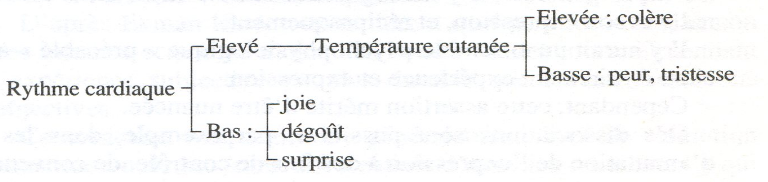
\includegraphics[width=10cm]{./Chapitre1/figures/Ekman1983.png}
  \caption{Traduction de la figure extraite de l'article de Paul Ekman et al.~\cite{Ekman1983} décrivant un arbre de décision pour déterminer l'émotion retrouvée sur le visage.}
  \label{fig:Ekman1983}
\end{figure}

  \item Il existe des éléments déclencheurs d'émotion qui sont universels : controversée, cette caractéristique stipule que des types de situations données provoqueront une émotion données chez tout sujet.
  \item Les réactions émotionnelles sont cohérentes : il y a un lien établi et connu entre une expérience émotionnelle et son expression physiologique et réciproquement.
  \item L'émotion engendre une réaction rapide : une fraction de seconde pour les réactions physiologiques et quelques millisecondes pour les mimiques~\cite{Ekman1978}.
  \item L'émotion est limitée dans le temps : la durée d'une émotion n'excède pas la minute.
  \item L'émotion n'est pas contrôlée : une émotion frappe soudainement, n'étant ni volontaire ni raisonnée. Un individu peut essayer de contrôler les manifestations de l'émotion. La posture et les mimiques sont plus contrôlables que la voix. Les réactions viscérales sont quant à elle très peu contrôlables.
  \item L'émotion est spontanée : elle n'est pas choisie et ne peut pas vraiment être éviter. Toutefois son anticipation peut réduire son intensité. Par exemple devant un film d'horreur, on s'attend à avoir peur, ce qui permet de réduire cette peur.
\end{itemize}

\begin{figure}
  \centering
  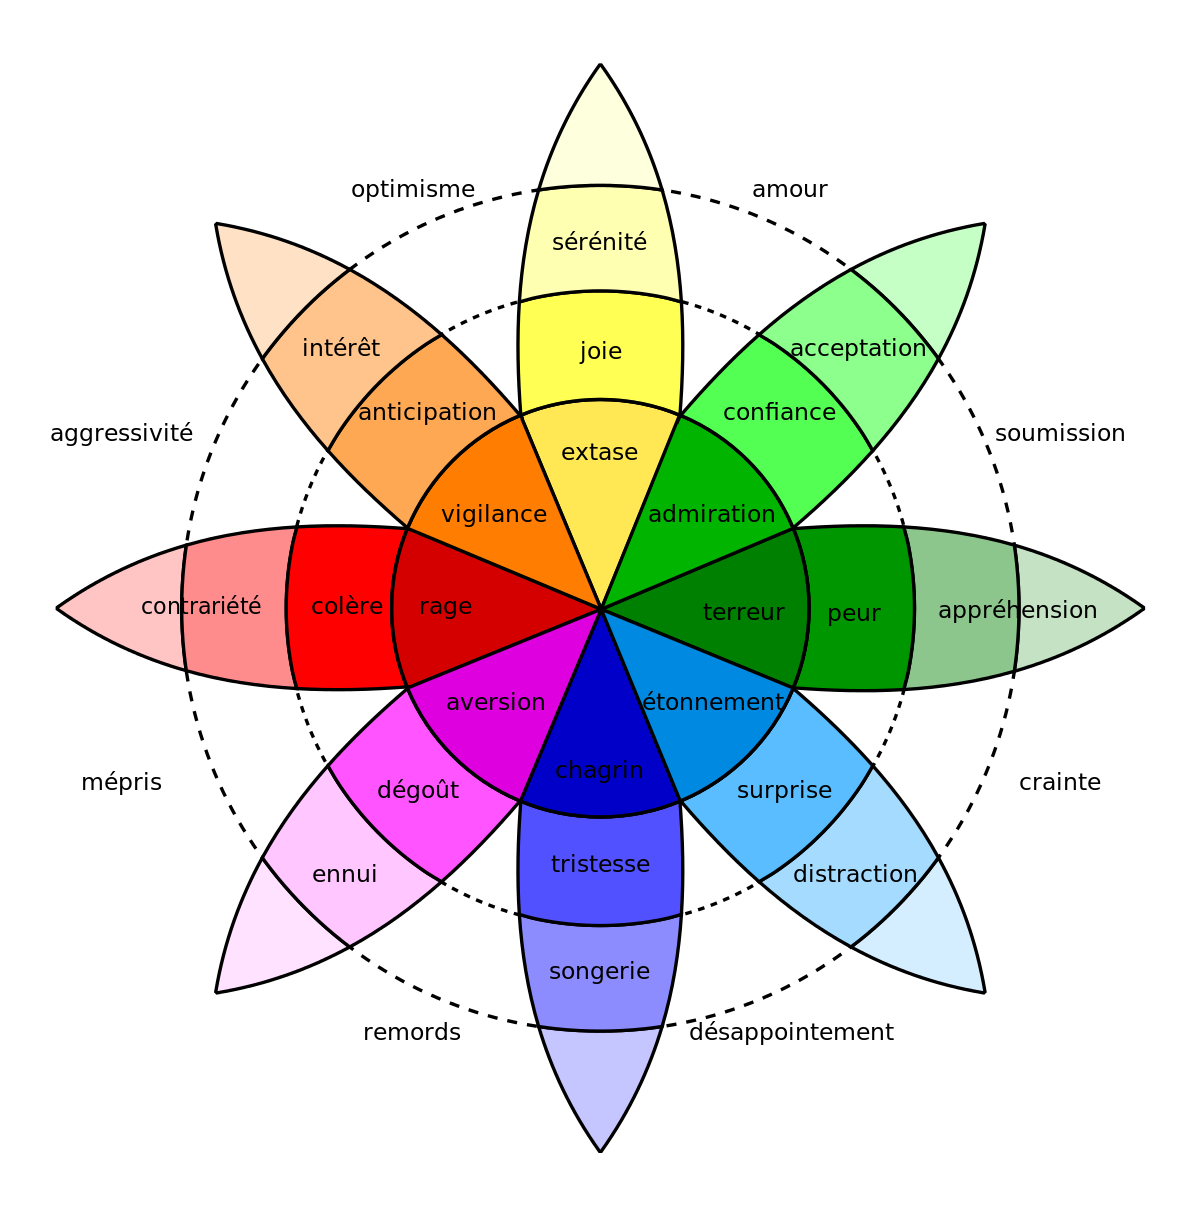
\includegraphics[width=12cm]{./Chapitre1/figures/Plutchik.png}
  \caption{Roue de Plutchik qui définit les émotions complexes à partir d'émotions basiques.}
  \label{fig:Plutchik}
\end{figure}


Ces émotions primaires peuvent également se combiner pour donner des émotions dites "complexes", qui permettent de nuancer les états émotionnels. C'est notamment le cas avec la roue de Plutchik, présentée dans la figure~\ref{fig:Plutchik}, qui dénombre 32 émotions caractérisées en 8 émotions primaires selon leur intensité~\ref{Plutchik1980}. De plus, on parle également d'émotions secondaires afin de décrire des émotions qui ne sont pas innées, mais qui sont apprises pendant le développement de la personne. Paul Ekman définit ainsi 9 émotions secondaires, plus complexes et plus difficiles à identifier (la culpabilité, l'embarras, le mépris, la complaisance, l'enthousiasme, la fierté, le plaisir, la satisfaction et la honte) qui sont marquent des différences d'expression en fonction des cultures et des individus. Charland (1995)~\cite{Charland1995} et Damasio (1999)~\cite{Damasio1999} ont notamment contribué à analyser les différences culturelles de ces émotions secondaires.
En plus de ces théories discrètes, l'émotion peut être définie par de nombreuses théories continues.

\subsection{Théorie des émotions continues}

\begin{figure}
  \centering
  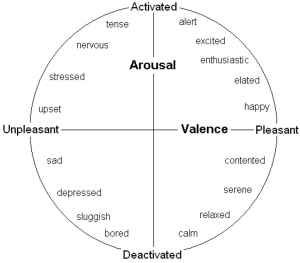
\includegraphics[width=8cm]{./Chapitre1/figures/Circumplex.png}
  \caption{Le modèle circumplex de Russell}
  \label{fig:Circumplex}
\end{figure}

Dans la vie courante, il est bien plus facile et coutumier de se référer à des catégories d'émotion tel que la joie ou la tristesse pour décrire ce que l'on ressent. Toutefois, une autre façon de définir les émotions est de les inscrire dans des espaces continus, permettant de s'affranchir des contraintes de ces catégories définies. Si l'on s'en réfère aux travaux de Feldman-Barrett (2006)~\cite{Feldman2006} , ces catégories «représente(nt) maintenant un obstacle majeur à la compréhension de ce que sont les émotions et de comment (les émotions) fonctionnent».
La théorie des émotions continues, aussi appelée émotions en dimensions, a été introduit par les travaux de Wundt (1902)~\cite{Wundt1902} et Schlosberg (1954)~\cite{Schlosberg1954}. Les émotions sont descriptibles selon trois dimensions indépendantes nommées en fonction de leur extremum : agréable-désagréable, tendu-détendu et agité-calme. Grace à ces trois dimensions, chaque émotion ressentie par un individu peut être décrite comme une combinaison pondérée de ces trois axes.  Comme ces dimensions se chevauchaient, ces dernières ont été remplacées par le modèle du Circumplex, présentée dans la figure~\ref{fig:Circumplex}, de Russell en 1980~\cite{Russell1980}, devenant la théorie principale permettant de décrire les émotions de façon continue. Ce modèle permet de placer toutes les émotions au sein d'un cercle dont l'abscisse définit la valence de l'émotion (positive-négative) et l'ordonnée définit l'activation (faible-fort). En effet, on peut donc donner une polarité et une intensité à chaque émotion. Afin de mieux discriminer des émotions qui avaient des mêmes valeur de valence et d'activation comme par exemple la peur et la colère, d'autres axes ont également été ajoutées sur ce modèle par Scherer (2005) comme la dominance (dominance-soumission), l'imprévisibilité (faible-forte)~\cite{Scherer2005}, comme illustré dans la figure~\ref{fig:Genova}. Par exemple, on peut voir que la mélancolie (melancholic) a une valence neutre et une faible activation, tandis que la déception (disappointed) a une valence très négative et une activation neutre.
\begin{figure}
  \centering
  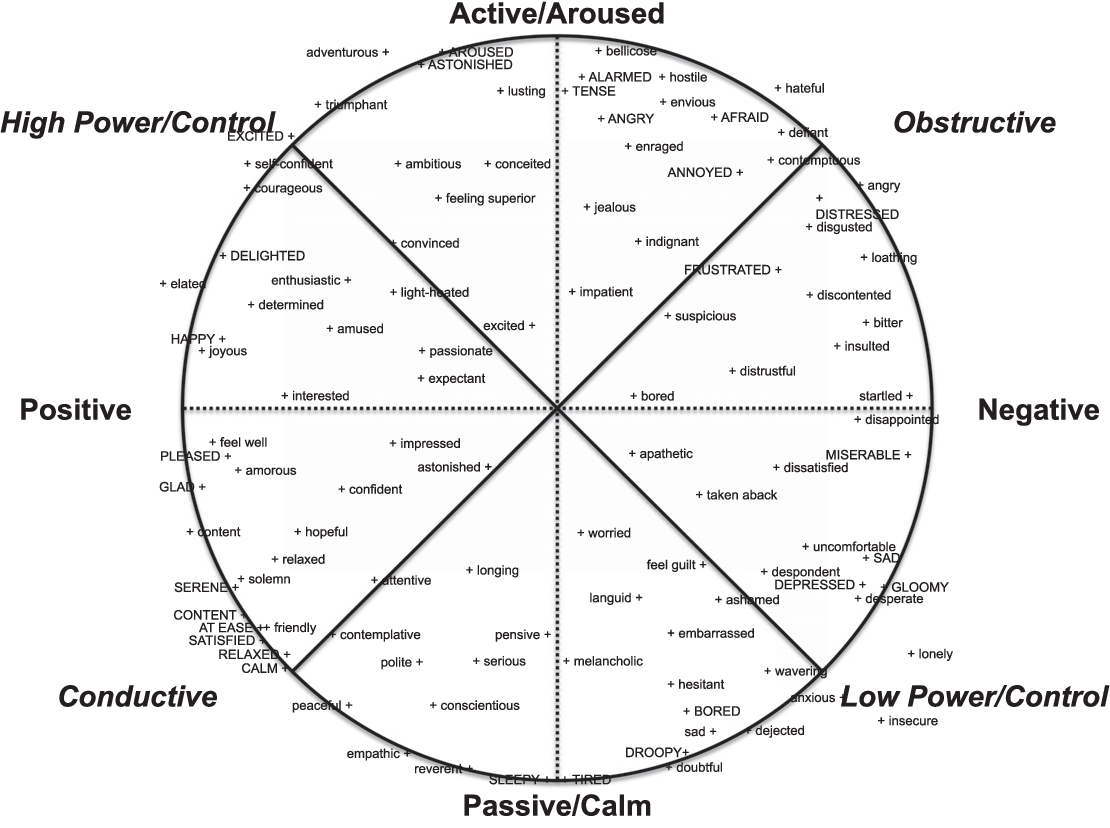
\includegraphics[width=18cm]{./Chapitre1/figures/Genova.png}
  \caption{La roue des émotions de Genève définie par Scherer, qui nomme des émotions (primaires ou secondaires) dans des dimensions continues.}
  \label{fig:Genova}
\end{figure}

D'autres systèmes dimensionnelles existent, allant de 2 dimensions à 5 dimensions, qui ont été crée en fonction des besoins applicatifs. Toutes ces dimensions peuvent être discrétisées par des systèmes de graduations, permettant notamment de faire le lien avec les théories discrètes.
En ce qui concerne les études menées sur les émotions continues dans le domaine de l'informatique, il y a une forte prévalence des dimensions de valence et d'activation quelque soit le support utilisé (la voix, le texte, la vidéo ou des données physiologiques). En effet, elles sont facilement identifiables par l'humain et reposent sur des caractéristiques automatiquement reconnaissables. Au sein de cette thèse, nous avons décidé de nous appuyer sur la théorie des émotions continues, afin de répondre à la problématique industrielle.


\section{L'émotion dans la parole : para-linguistique et prosodie}
Si nous nous replaçons dans le contexte de cette thèse, notre objectif est de décrire l'émotion humaine lors de conversations tenues entre un client et un agent dans un cadre défini par un appel téléphonique en centre d'appels. Nous n'avons donc que la voix comme axe d'analyse pour en retirer les états émotionnels des intervenants.
La voix, produite par l'appareil phonatoire humain, que l'on considère comme un canal de communication comme définit par Shannon (1948)~\cite{Shannon1948}, permet de faire passer un message entre un émetteur (ici le locuteur) et un récepteur (ici l'écoutant) grâce à son appareil auditif.

Ces deux appareils sont la base de la communication orale entre deux individus. L'appareil phonatoire décrit l'ensemble des phénomènes anatomiques qui sont impliquées dans la production des vibrations acoustiques donnant naissance à la parole. Par exemple, la création d'un son par la vibrations des cordes vocales ou encore la modulation de ce son par la bouche et le nez. La parole peut etre découper en sous unité phonique que l'on appelle des phonèmes. Ces derniers, à ne pas confondre avec des syllabes, permettent de composer l'ensemble des sonorités nécessaires à l'énonciation de parole.
%Par exemple, le mot 'émotion' utilise 6 phonèmes : /e/ (é), /m/ (m), /ɔ/ (o), /s/ (s), /i/ (i) et /ɔ̃/ (on).
Le langage étant directement influencé par la langue parlée par le locuteur, chaque langue possède sa propre palette de phonèmes. Le français par exemple utilise 37 phonèmes, tandis que le japonais n'en utilise que 22.
L'appareil auditif quant à lui, est composé de tout ce qui permet à l'individu d'entendre et d'écouter la parole. Il est notamment composé de l'oreille mais également du cerveau, qui est un acteur de la perception auditive. Pour ce qui est de l'oreille, elle se compose de trois parties :
\begin{itemize}
  \item l'oreille externe : conduit qui permet de transmettre les vibrations acoustiques
  \item l'oreille moyenne : transforme le signal pour qu'il puisse être conduit dans un environnement liquide en utilisant les osselets,
  \item l'oreille interne : transforme les vibrations en influx nerveux grâce à la cochlée.
\end{itemize}
C'est cet appareil qui permet à un interlocuteur de recevoir un message.

Les informations communiquées par ce canal peuvent être notamment divisées en deux catégories, la linguistique et le para-linguistique.
Le linguistique va décrit le langage en tant que parole de base tandis que le para-linguistique va définit tout ce qui n'est pas du message verbal. Par exemple, dans la vie de tous les jours, "Bonjour, je voudrais une baguette de pain" correspond au message linguistique, tandis que le sourire, le geste de la main, l'hésitation vocale ou le raclement de gorge fera partie du domaine para-linguistique.
Shirley Weitz (1974)~\cite{Weitz1974} explique que la paralinguistique s'intéresse "à la façon dont quelque chose est dit, pas à ce qui est dit". Globalement, on considère du domaine du para-linguistique dans la parole, l'accent, la hauteur, le volume, la vitesse de parole, la modulation, la prosodie et la fluidité de l'élocution.
La définition du paralangage étant évolutive, il est donc naturellement que sa définition reste imprécise comme l'indique Peter Matthews dans son dictionnaire de la linguistique~\cite{Matthews2014}.
La prosodie est défini par l'ensemble des phénomènes qui accompagnent le discours, tout en n'étant pas du discours. Elle est notamment marquée par trois paramètres très important:
\begin{itemize}
  \item La fréquence fondamentale (F0) de la parole correspond à l'inverse de la période d'un son périodique, c'est à dire à la durée des sons de type voyelles dans la parole,
  \item La rythme de la parole qui correspond au temps nécessaire à l'émission d'un segment de parole,
  \item l'intensité de la parole qui est définit par l'énergie contenue dans le signal.
\end{itemize}
C'est par l'étude para-linguistique et de la prosodie que nous analysons notamment inconsciemment le discours d'un locuteur afin de déterminer son état émotionnel. Comme il s'agit du sujet principal de cette thèse, le chapitre~\ref{chapitre3} revient plus en détail sur la relation entre la voix et les émotions. Mais la voix n'est pas la seule modalité véhiculant des indices émotionnels.

\subsection{Satisfaction et frustration dans la voix}

\section{L'émotion dans le texte}
Utiliser le texte pour déterminer l'état émotionnel est une voie de plus en plus empruntée grâce, notamment, à la performance des systèmes de reconnaissance de la parole actuel.
Si des domaines comme l'Affect analysis ou la détection d'opinion utilise des données textuelles de type livres, témoignages ou plus récemment tweets et contenus en ligne afin d'extraire des états émotionnels, on peut également considérer la transcription automatique comme un élément dissocié de la parole, et donc y retrouver des marqueurs de l'émotion. Rappelons que l’analyse de sentiments désigne plutôt l’analyse en polarité positif-négatif de l'occurence, tnadis que l'opinion est généralement décrites en trois catégories "bien/neutre/mal".On cherche alors l'émotion dans l'aspect sémantique de la phrase, dans les diffluences ou les répétitions.
Des outils tel que des dictionnaires de polarité permettent de colorer émotionnellement des mots ou des phrases, ou encore des postagger permettant d'étudier la structure d'un énoncé pour faire ressortir sa forme morphosyntaxique sont utilisés dans la reconnaissance d'émotions que ce soit à l'échelle d'un segment de parole, d'une phrase ou d'un document.

\subsection{Satisfaction et frustration dans le texte}

\section{Les autres indices émotionnels chez l'humain}
Outre la présence de marqueurs émotionnelles dans la voix, d'autres indicateurs peuvent être relevées dans notamment les expressions faciales et les signaux physiologiques. Il est donc possible d'étudier l'état émotionnel d'une personne à partir d'une vidéo ou de relevés cardiaques par exemple.

\subsection{Les marqueurs faciaux et comportementaux de l'émotion}

\begin{figure}
  \centering
  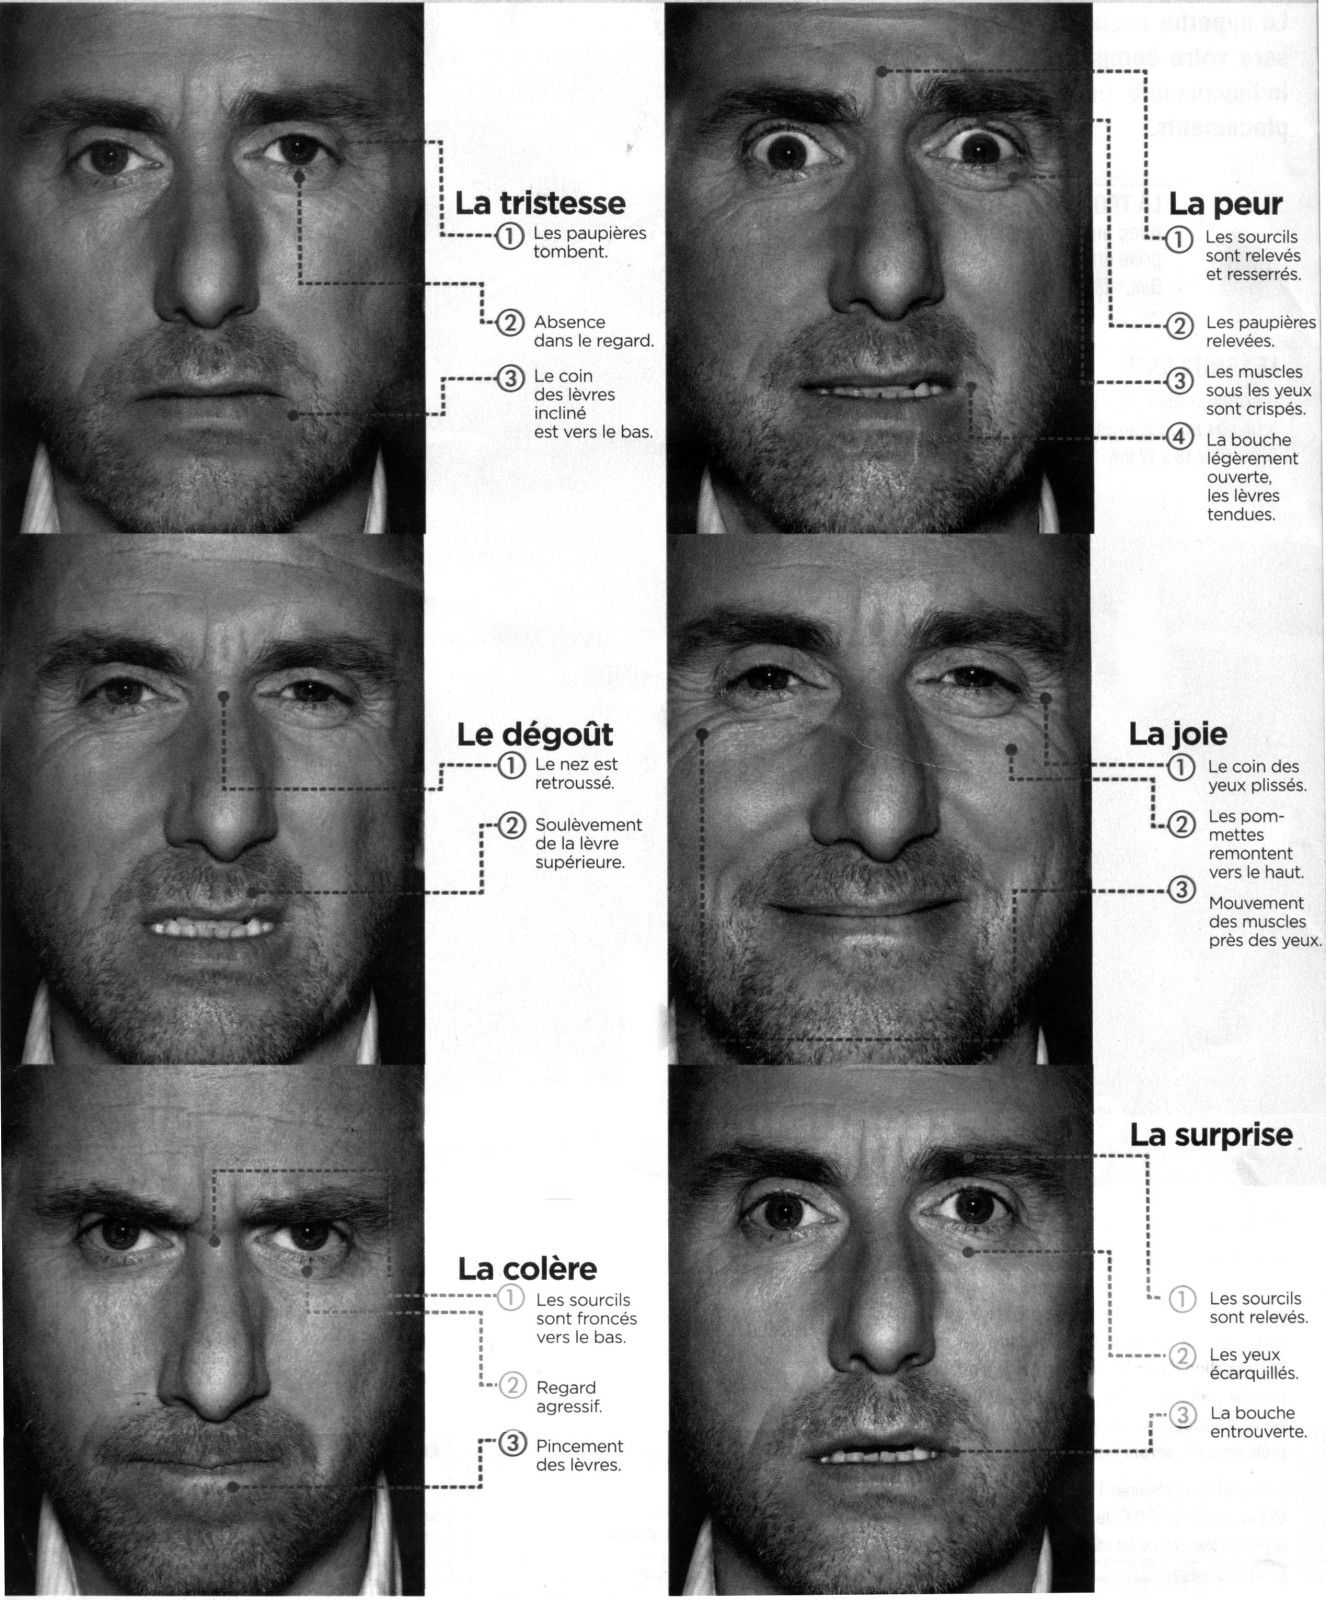
\includegraphics[width=14cm]{./Chapitre1/figures/ExpressionFacial.jpg}
  \caption{Marqueurs faciaux des 6 émotions primaires d'Ekman. In Lie To Me.}
  \label{fig:expressionFacial}
\end{figure}

Il est possible de capter beaucoup d'information sur le visage et dans l'attitude d'une personne. Nos expressions faciales notamment permettent de véhiculer les émotions primaires tel que la peur ou la colère~\ref{fig:expressionFacial} en mettant en jeu le positionnement des sourcils, la forme de la bouche, le plissement du front... Bien qu'affirmé comme étant universelles par Paul Ekman~\cite{Ekman1978}, de nombreuses études ont mis en doute ce postulat. En effet, certains indicateurs étant communs entre plusieurs émotions, des interlocuteurs peuvent se tromper dans l'analyse de l'émotion de la personne. Par exemple, la bouche ouverte peut signifier la peur mais également la surprise. Les expressions faciales sont également contrôlables. En effet, il est tout à fait possible de simuler une émotion ou dans une moindre mesure, d'en cacher une selon l’entraînement d'un individu.
Malgré ces inconvénients, les expressions faciales sont, aujourd'hui encore, l'une des modalités les plus observées pour définir et reconnaître des émotions. Elles peuvent également servir à détecter des états dépressifs ou des mensonges par exemple.

L'attitude d'une personne permet également de reconnaître ces émotions. En effet, les comportements adoptés par un individu, notamment la posture, peuvent refléter de l'état émotionnel interne d'une personne. Ce phénomène est expliqué dans les travaux de Fijda (1987)~\cite{Fijda1987} qui indique que les émotions sont la pour aider l'homme à agir : l'homme est caractérisé par une tendance à l'action qui se traduit par des émotions. Ainsi lors de la colère, la position du buste du corps sera en avant, tandis que pour la peur, elle sera recroquevillée sur elle-même. Mais ces marqueurs faciaux et comportementaux ne sont pas les seuls marqueurs utilisables.

\subsection{Les marqueurs physiologiques de l'émotion}
Comme nous l'avons vu précédemment, l'expression de l'émotion est étroitement liée au cerveau et donc au système nerveux. En étudiant ce dernier, nous pouvons retrouver des marqueurs émotionnels. La peur par exemple, engendre une augmentation du rythme cardiaque, qui va augmenter l'afflux sanguin, de la sudation, l'augmentation de l'apport en oxygène par une respiration plus rapide. De manière non-exhaustive, nous pouvons citer le rythme cardiaque, la sudation, la température de la peau (à l'origine des joues rouges), l'activité cérébrale, le suivi du regard, le rythme de la respiration comme des marqueurs physiologiques de l'émotion. Certains de ces marqueurs physiologiques peuvent être quantifiés par des outils de mesure. L'électrocardiogramme (EG) permet de suivre l'évolution du rythme cardiaque, l'électroencéphalogramme (EEG) permet de détecter les zones d'activités du cerveau. Des capteurs de sudation et des thermomètres peuvent permettre de suivre la production de sueurs au niveau des main ou la température corporelle. Tous ces indicateurs peuvent caractériser la présence ou l'absence d'émotion chez un individu ainsi que la caractériser.
